	El núcleo del Kit de Desarrollo FX2LP EZ-USB es un CY7C68013A. Dicho circuito integrado, cuya arquitectura se presenta en la Figura \ref{arqEzUSB}. Los chips de la familia FX2LP integran un transceptor USB, un SIE {\it Serial Interfaz Engine}, buffers de datos, un microcontrolador 8051 mejorado y una interfaz programable hacia los periféricos. Además posee un un PLL y un divisor configurable a través de los cuales provee al sistema de una señal de reloj adecuada para el correcto funcionamiento del sistema.\\
	
	\begin{figure}[b]
		\centering
		%TODO meter la imagen
		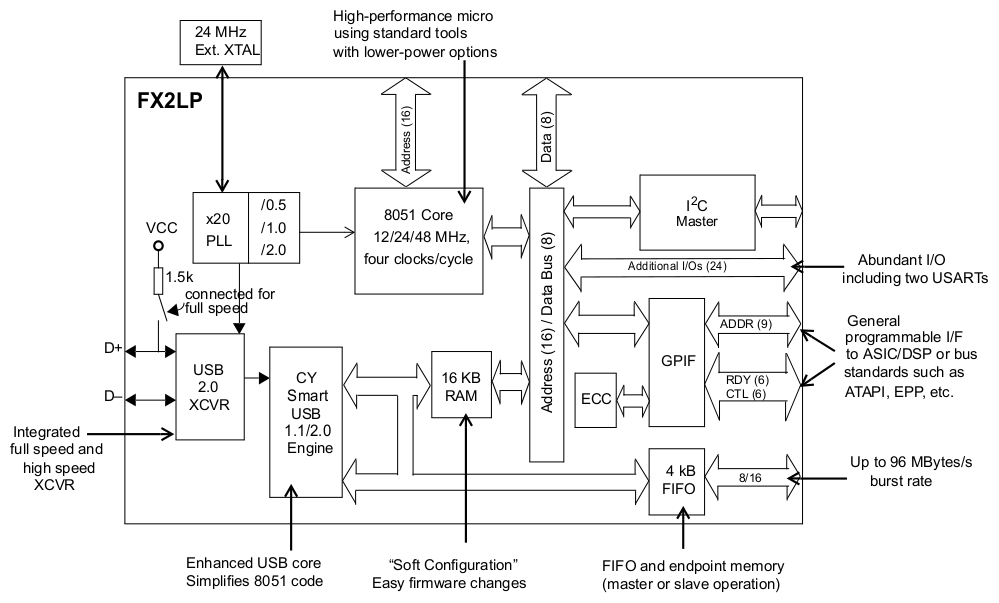
\includegraphics[width=.7\textwidth]{arqfx2lp.png}
		%TODO Meter la referencia
		\caption{Arquitectura FX2LP} 
		\label{arqEzUSB}
	\end{figure}

	La arquitectura que posee el integrado permite al usuario trasmitir datos desde y hacia la PC desde el mimso puerto USB, o bien via RS-232, desde la PC. A la hora de comunicarse con sistemas periféricos se puede aprovecar el puerto I2C, la interfaz de propósito general o una interfaz esclavo que puede ser conectada a un sistema maestro. Esto brinda muchas alternativas, desde la conexión a puertos estandar, como ser ATA o PCMCIA, EPP, como también la conexión de dispositivos tales como DSP's y FPGA's.\\
	
	El esquema de bus permite utilizar el microcontrolador 8051 para procesar datos, hacer control de errores, empaquetar datos de una forma particular, generar datos nuevos, entre otras, o bien, simplemente enviar datos desde un periférico de forma directa al SIE y luego transmitirlos a la PC por la tubería USB.\\
	
	Para este trabajo final, se utilizó la función maestro esclavo, a través de la memoria FIFO destinada para tal fin. Por lo que se describirá en detalle a continuación.
	
	La memoria FIFO de 4kB se conecta de forma directa a los periféricos y es configurable, lo que permite al usuario disponer del espacio conforme requiera las necesidades de ancho de banda de los sistemas diseñados, evitando así las congestiones en casos de mucho flujo de datos. En el otro extremo, puede ser conectada al tubo USB o al microntolador.\\ 
	
	